% !TeX encoding = UTF-8
\section{Umsetzung}
\label{sec:Umsetzung}
Es gibt unterschiedliche Vorgehensweisen, einen RRT* zu bauen und neu zu verknüpfen. Besondere Bedeutung hat dabei, wie neu erzeugte Knoten dem Baum hinzugefügt werden. Mein in der Einleitung erwähnter Kommilitone David Gödicke benutzte in seiner Bachelorarbeit zum Erreichen zweier Punkte innerhalb des Baumes Dubin curves \citep{Dubin61} beziehungsweise Reed Sheep curves \citep{reeds1990optimal}, sodass der neu hinzugefügte Knoten stets durch seinen Vater erreichbar war \citep{Goedicke18}. Leider war die Berechnung dadurch insgesamt zu aufwändig und langsam, was für Echtzeit-Szenarien im Straßenverkehr ein hartes Ausschlusskriterium ist, weshalb Goedicke diesen Ansatz nicht empfehlen konnte \citep[vergleiche][Kapitel 7]{Goedicke18}. \\
Daher entschloss ich mich, Varianten von RRT* zu untersuchen, bei denen das Auto direkt von Knoten zu Knoten fährt. Dadurch benötigt es nur eine Lenkeinstellung zwischen zwei Knoten und die Berechnung wird einfacher.\\
\begin{figure}
\label{fig:reachable}
\centering
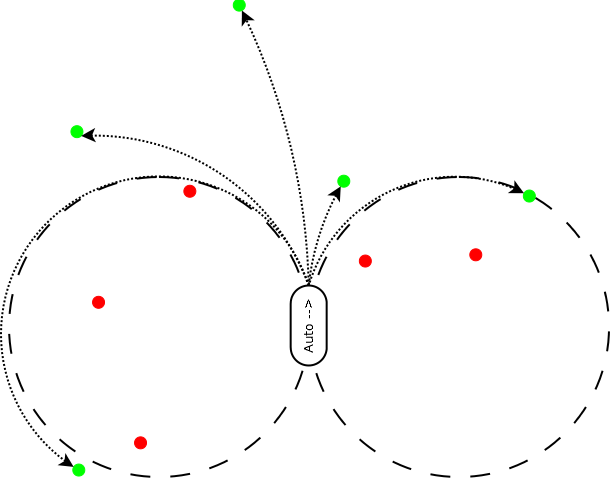
\includegraphics[scale=0.5]{Bilder/Erreichbarkeit_Punkte.png} 
\caption{Erreichbare und nicht erreichbare Punkte vom Auto aus}
\end{figure}
\subsection{Übersicht}
Hier werden vier verschiedene Ansätze vorgestellt, mit deren Hilfe das Auto mit dem RRT* Algorithmus von der Startposition in den Zielbereich kommt.
\begin{enumerate}
\item Erster Ansatz: Nicht erreichbare Knoten werden dem Baum nicht hinzugefügt. Kostenfunktion berücksichtigt Lenkänderungen. Rewiring findet Rekursiv statt.
\item Zweiter Ansatz: Alle Knoten sind erreichbar, aber nur außerhalb der Wendekreise. Kostenfunktion berücksichtigt Lenkänderungen.
\item Dritter Ansatz: RRT* ohne Einschränkungen durchgeführt, das heißt alle Knoten sind gültig. Am Ende wird ein Pfad vom Ziel zum Startknoten erstellt, der abfahrbar ist.
\item Vierter Ansatz: Nicht erreichbare Knoten werden dem Baum nicht hinzugefügt. Kostenfunktion berücksichtigt Lenkänderungen. Rewiring wird nur bei dem Knoten mit der besten Kostenersparnis durchgeführt.
\end{enumerate}
Diese 
 Dabei müssen diese Ansätze folgende Bedingungen erfüllen: \\
\begin{enumerate}
\item Garantie der Abfahrbarkeit: Das Auto muss in der Lage sein, der berechneten Trajektorie zu folgen. Da das Auto die Punkte innerhalb der Wendekreise nicht erreichen kann(siehe \ref{fig:reachable}), muss sichergestellt werden dass diese Punkte nicht als Kindknoten gewählt werden können.
\item Geringe Kosten: Es muss nicht der optimale Pfad gefunden werden, aber er sollte zumindest asymptotisch optimal sein. 
\item Niedrige Berechnungsdauer: Da der Algorithmus mehrmals pro Sekunde ausgeführt werden soll, sind Ausführzeiten über 250 Millisekunden nicht tolerierbar. Bei Messungen der Ausführzeit muss jedoch auch die Wahl der Datenstruktur, Metrik und die Art der Implementierung berücksichtigt werden, da diese zusätzlich die Laufzeit verändern können.
\end{enumerate}
Die vier Ansätze werden anhand der obigen Kriterien untersucht und bewertet.

\begin{enumerate}


\subsection{Erster Ansatz}

\item Erster Ansatz: Einen Baum mit RRT* erzeugen, ohne die kinematischen Einschränkungen des Autos zu berücksichtigen. Durch die Eigenschaften des RRT* werden gerade Pfade erzeugt, deren Abfahren kein Problem ist. Wenn Ecken unvermeidbar sind (z.B. beim Herumfahren um Hindernisse) wird durch eine Heuristik dafür gesorgt, dass der Pfad abfahrbar bleibt.
\item Einen Baum mit RRT* erzeugen. Wenn Erzeugung abgeschlossen: Pfad zum Ziel so bearbeiten, dass dieser vom Auto zu bewältigen ist (keine Ecken)
\item Einen Baum mit RRT* erzeugen, aber nur Knoten hinzufügen, die von ihrem Vaterknoten aus unter oben genannten Bedingungen stets erreichbar sind

\end{enumerate}
Das Problem des ersten Ansatzes war, dass unter Umständen, je nach Umgebung, ein Pfad nicht abfahrbar ist. Nicht abfahrbar heißt, dass der Pfad Ecken und Kurven besitzt, die aufgrund des Lenkradius des Autos nicht zu bewältigen wären. Es wäre zwar möglich, für kurze Zeit die geplante Trajektorie zu verlassen und nach Ende der Kurve wieder zu ihr zu stoßen, allerdings ist es unter diesen Umständen schwierig eine Hindernisfreiheit zu garantieren. \\
Der zweite Ansatz ist zwar prinzipiell möglich. Ziel des ganzen war jedoch, wie in Kapitel \ref{sec:Problemanalyse} geschildert, das Neuplanen und überprüfen der Trajektorie auf Gültigkeit in einem engen Zeitfenster um auf dynamische Hindernisse zu reagieren. Dies ist mit einem Bearbeiten des Pfades vom Ziel zum Startknoten ineffizient und aufwändig.\\
Deshalb entschloss ich mich zuerst für die dritte Variante, bei der Knoten nur zum RRT*-Graph unter der Bedingung hinzugefügt werden, dass sie erreichbar sind.
\subsubsection{Vorauswahl}
\label{sec:Vorauswahl}
[TODO ist eig alles veraltet, muss neu geschrieben werden. Ich kann mit dem Auto jetzt jeden Punkt außerhalb der Wendekreise erreichen...damit fällt alles mit Erreichbarkeit über den Winkel weg,alles andere wie Projektion, Berechnung der Orientierung und Sicherstellen-das-der-Knoten-nicht-zu-nah-ist bleibt aber bestehen...\\
Vor allem müssen neue Grafiken erstellt werden (Mi?)!]
Diese beinhaltete, bei der Erstellung des RRT* vom Auto nicht erreichbare Knoten gar nicht erst zuzulassen. Das Auto sollte also von einem Knoten zum nächsten mit nur einer Lenkeinstellung direkt fahren können. Dies sollte die Berechnungszeit stark verringern. \\
Zum Ausschluss der Knoten verwendete ich zuerst eine Heuristik: Ein nächster Nachbar N für einen neu hinzugefügten Knoten K kam nur dann in Frage, falls dieser den neu hinzugefügten Knoten K auch erreichen konnte. Dazu wurde die Ausrichtung des Autos im potenziellen Elternknoten N mit dem Richtungsvektor zwischen den beiden Knoten verglichen. Somit war K gültig, falls der Winkel zwischen der Ausrichtung von N und dem direktem Weg zum Knoten K (Richtungsvektor) einen bestimmten Wert $\gamma$ nicht überschritt.
\begin{figure}
\centering
\label{fig:fig4}
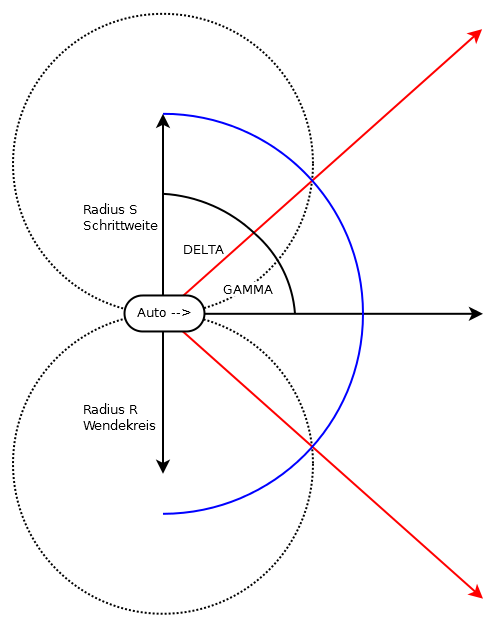
\includegraphics[scale=0.6]{Bilder/AusrichtungGrob.png} 
\caption{Bedeutung der Schrittweite und Radius für den Winkel Gamma}
\end{figure}
 $\gamma$ direkt zu berechnen war nicht ohne weiteres möglich, doch mit Hilfe des Kosinussatzes konnte der Winkel $\delta$ (siehe Abbildung ~\ref{fig:fig4}) berechnet werden. Dieser berechnet sich aus dem Radius $R$ des Wendekreises des Autos und der verwendeten Schrittweite, also dem maximalen Abstand zwischen zwei Knoten. \\
Der Knoten K konnte wurde im ersten Schritt als gültig erkannt, wenn für die Differenz zum Winkel des Elternknoten galt: 
\begin{center}
$diff(K,N) <\gamma$ \\
$\gamma = 90^{\circ} - \delta$  \\
$\delta = arccos (\frac{Schrittweite}{2 \dot R})$  \\
\end{center}

Alle Knoten außerhalb dieses Winkels würden bei der Projektion im Wendekreis des Autos landen, wie in Abbildung \ref{fig:fig5} zu sehen. Diese Knoten(rot) wurden verworfen.\\
\subsubsection{Projektion}
Als nächster Schritt wird, wie in Kapitel \ref{RRT*} geschildert, der Knoten K an den nächsten (gültigen) Nachbarn N projiziert und der Vaterknoten bestimmt. Sollte der Knoten näher am Vaterknoten dran sein, als die Schrittweite ist, wird der Knoten nicht projiziert, da sonst alle Knoten zu ihrem Vaterknoten den gleichen Abstand hätten und bestimmte Bereiche somit nicht auf optimalen Weg erreichbar wären. Da innerhalb der Schrittweite durch den maximalen Lenkwinkel des Autos selbst die Knoten, die vom Winkel her gültig sind, nicht erreichbar sein können ist eine zusätzliche Überprüfung für diese Knoten notwendig. \\
Da der maximale Lenkwinkel eines Autos vorgegeben ist hängt also die Erreichbarkeit des Knotens allein von der Schrittweite ab. Mit dieser kann auch vorgegeben werden, wie um wie viel Grad sich die Ausrichtung des Autos bei einem Schritt ändern darf und ob beispielsweise Kehren erlaubt sind. Dabei muss jedoch beachtet werden: Bei einer zu kleinen Schrittweite werden viele Knoten verworfen und es werden kaum enge Kurven möglich sein. Bei einer zu großen Schrittweite werden sehr kurvige Trajektorien entstehen, sodass z.B. Hinderniserkennung nicht mehr so einfach ist.
\begin{figure}
\centering
\label{fig:fig5}
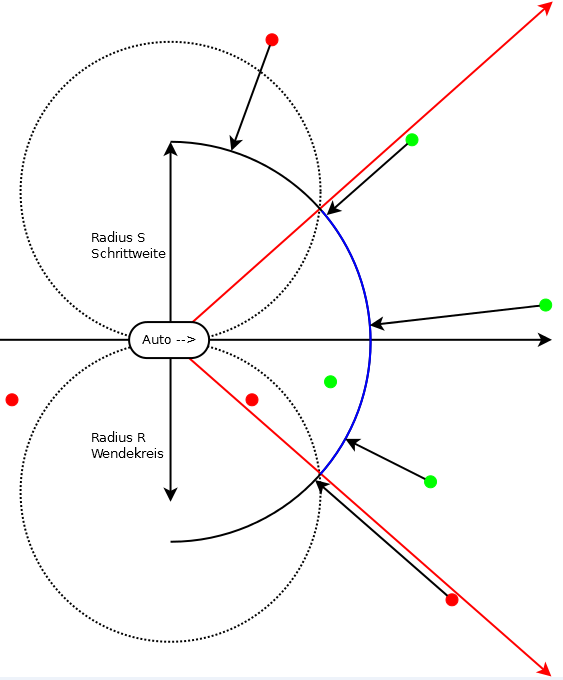
\includegraphics[scale=0.7]{Bilder/Projektion_der_Punkte.png} 
\caption{Projektion der Punkte auf Schrittweite}
\end{figure}
\subsubsection{Bestimmung des Vaterknotens}
Nachdem der Knoten an seinen nächsten Nachbarn projiziert wurde, wird nun aus allen nächsten Nachbarn innerhalb eines Radius R der mit den besten Kosten gewählt. Im Verfahren zur Bestimmung des nächsten Nachbarn, siehe \ref{sec:Vorauswahl}, wurden nicht beachtet dass der neue Knoten innerhalb der Wendekreise des Autos liegen könnte. Es ist dem Auto aber nicht möglich, vom Vaterknoten N zum Knoten K zu fahren, wenn K im Wendekreis des Autos liegt. \\
Für jeden Knoten im Radius R wird geprüft, ob dieser Knoten unseren neuen Knoten K erreichen kann. Das wird ausgerechnet, indem vom potentiellen Vaterknoten N aus zwei Mittelpunkte der Wendekreise bestimmt werden. Wenn der Abstand von K zu diesen Mittelpunkten kleiner ist als der Radius der Wendekreise, liegt K im Wendekreis und ist nicht erreichbar. Damit kommt N als Nachbar nicht in Frage. Falls kein nächster Nachbar im Radius R den Knoten K erreichen kann, wird K verworfen. \\
Nachdem erfolgreich ein Vaterknoten bestimmt und dem neu hinzugefügtem Knoten K zugewiesen wurde, muss noch die Ausrichtung oder Orientierung bestimmt werden, die das Auto im Knoten K hat.
\subsubsection{Bestimmung der Orientierung}

\begin{figure}
\label{fig:fig8}
\centering
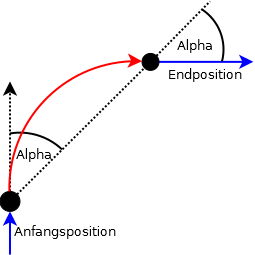
\includegraphics[scale=1]{Bilder/BerechnungOrientierung.png} 
\caption{Berechnung der Ausrichtung}
\end{figure}
Da das Auto im Vaterknoten N eine bestimmte Ausrichtung hat und mit nur einer Lenkeinstellung zum nächsten Knoten K gelangt, ist dort die Ausrichtung dadurch festgelegt und berechnet sich aus der Ausrichtung des Vaterknotens, Winkel $\theta$, und dem Winkel zwischen der Ausrichtung des Vaterknotens und dem Richtungsvektor von N nach K. Wie in der Zeichnung ~\ref{fig:fig8} zu sehen ist, berechnet sich die Ausrichtung $\omega$ des neuen Knotens K folgendermaßen:
\begin{center}
	$\theta + 2 \pi - 2*\alpha = \omega$
\end{center}
\subsection{Metrik und Kostenfunktion}
\label{sec:Metrik}
Eine besondere Bedeutung zur Erzeugung einer "guten" Trajektorie kommt der Kostenfunktion zu. Diese sorgt nicht nur dafür, welcher Knoten als Vaterknoten ausgewählt wird, sondern spielt auch beim Neuverknüpfen des Baumes eine Rolle.Somit kann mithilfe der Kostenfunktion für besonders gut abfahrbare oder besonders kurze Pfade gesorgt werden. \\
Da durch die Orientierung des Vaterknotens die Orientierung des Kindknotens bereits festgelegt ist (siehe Abbildung ~\ref{fig:fig8}, können aus eigentlich geraden Strecken sehr ungünstige Pfade entstehen.\\
 In Abbildung ~\ref{fig:fig5} wird als Kostenfunktion der euklidische Abstand benutzt. Knoten C wählt aus B1 und B2 den nächsten Nachbarn aus, das ist B2. Leider entsteht dadurch eine sehr kurvige Route, bei der vom fast maximalem Lenkeinschlag nach rechts auf den maximalen Lenkeinschlag der anderen Seite gewechselt werden muss. Neben Nachteilen des Komforts, der Sicherheit und längerem Weg wird auch die Ungenauigkeit höher. Anfangs wurde angenommen, dass der Lenkwinkel sich sofort ändern kann. Während bei kleinen Änderungen diese Annahme nur für kleine Fehler sorgt, sind die Auswirkungen bei solch starken Änderungen deutlicher spürbar.


\begin{figure}[htb]
  \label{fig:fig6}  
    \centering
    \begin{minipage}[t]{0.45\linewidth}
        \centering
        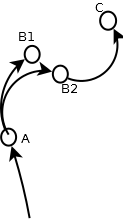
\includegraphics[width=.6\linewidth]{Bilder/B2Insert.png}
        \caption{einfache euklidischeKostenfunktion}
    \end{minipage}% <- sonst wird hier ein Leerzeichen eingefügt
    \hfill
    \begin{minipage}[t]{0.45\linewidth}
\label{fig:fig9}                 
        \centering
        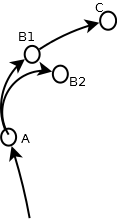
\includegraphics[width=.6\linewidth]{Bilder/B1Insert.png}
        \caption{erweiterte Kostenfunktion}
    \end{minipage}
\end{figure}


In Abbildung ~\ref{fig:fig9} hingegen wurde eine bessere Kostenfunktion gewählt, sodass über B1 gehend ein effizienterer, kürzerer Pfad entsteht. Die Kostenfunktion muss dabei die Ausrichtung des Autos beim Vaterknoten N berücksichtigen. [TODO Auswahl] Eine Möglichkeit wäre dann, die tatsächliche zu fahrende Strecke des Autos zu benutzen und dadurch effizientere Pfade zu bevorzugen. Eine andere Möglichkeit ist, zu harte Richtungsänderungen zu bestrafen und kleine $ \Delta \theta$ zu bevorzugen. \\
Als Lösung wurde hierbei eine Kombination aus dem euklidischem Abstand und der Winkeldifferenz der Knoten K und N zur Kostenberechnung zu benutzen. Die Kosten berechnen sich dann wie folgt: 
\begin{center}
$cost(K) = cost(N) +eukl. Abstand(K,N) * (1+Winkeldifferenz)$
\end{center} 
Bei einer geraden Strecke wird lediglich der euklidische Abstand als Kosten aufsummiert, bei einer Kehre von 180$^{\circ}$ bis zum vierfachen der euklidischen Kosten (Winkeldifferenz $\pi$ +1).\\
Nachteil dieser Kostenfunktion ist, dass nicht berücksichtigt wird das starke Kurven weniger "schlimm" sind auf größerer Strecke. Mit anderen Worten, das Fahren genau auf den minimalen Wendekreisen ist meist weniger angenehm als das Fahren auf weiten Kreisen, auch wenn beide Pfade die gleiche Winkeldifferenz haben. Das Problem hierbei ist, dass ein kleinerer Kreis geringere euklidische Kosten hat und demzufolge gegenüber dem größeren Kreis bevorzugt wird.
\subsubsection{Rewiring}
[TODO Rewiring neu schreiben, siehe oben. Hat sich geändert, Rewiring muss nicht Rekursiv durchgeführt werden.] 
Die Neuverknüpfung geschieht im RRT, indem, wie in \ref{sec:rewiring} geschildert, der Knoten K allen Knoten im Radius R hinzugefügt wird, bei denen er die Gesamtkosten verbessert. \\
Dadurch, das im Gegensatz zu einem normalen RRT* nun auch die Ausrichtung eine Rolle spielt, kann der Baum nicht ohne weiteres neu verknüpft werden. Wenn ein Knoten K mit Ausrichtung $\theta$ durch Rewiring einen neuen Vaterknoten bekommt, ändert sich $\theta$. Da aber sowohl die Erreichbarkeit der Kindknoten von K als auch die Kostenfunktion von $\theta$ abhängen, kann es sein, dass nun nicht mehr alle Kindknoten erreichbar sind. \\
Die erste Lösung zu diesem Problem wäre, die Ausrichtung des Knotens K nicht zu ändern, sondern einen neuen Knoten mit gleichen Koordinaten, aber anderer Ausrichtung hinzuzufügen. Da wir einen neuen Knoten hinzugefügt haben, müssen wir nun auch erneut die Rewiring Operation durchführen. Somit entsteht mit jedem neu hinzugefügten Knoten ein Wasserfalleffekt durch den ganzen Baum, welcher im schlechtesten Fall eine exponentielle Laufzeit hat - ein nicht tragbares Szenario für eine Echtzeitanwendung. \\
Theoretisch kann ein Auto mit nur einer Lenkeinstellung alle Punkte außerhalb der Wendekreise erreichen. Das Problem der Nichterreichbarkeit könnte also dadurch behoben werden, dass nur Knoten in einem bestimmten Abstand als Vaterknoten erlaubt sind. Die dadurch entstehenden schlechte Trajektorien (z.B. mit 180$^{\circ}$ Kurven) können nicht durch die Wahl einer geeigneten Kostenfunktionen vermieden werden, da die Kostenfunktion auch vom Winkel $\theta$ abhängt - und dieser ist veränderbar. \\
Deshalb werden für das Rewiring zwei Möglichkeiten vorgeschlagen:
\begin{enumerate}
	\item Schlechte Trajektorien werden toleriert, Nichterreichbarkeit durch entsprechende Abstände vermieden [TODO d.h. man überall die gleichen Abstände bzw. Abstände zwischen 2*Lenkradius und Schrittweite]
	\item Die oben geschilderte Rewiring-Operation wird durchgeführt, allerdings nicht mit allen erreichbaren Knoten im Radius, sondern nur bei dem Knoten, bei denen der Effekt am größten ist, also durch das Rewiring am meisten Kosten gespart werden [TODO Bild zeichnen und einfügen]. Bei dem so neu hinzugefügten Knoten wird auch wieder die Rewiring-Operation durchgeführt, bis ....und hier kam die Erkenntnis: Bis wann eigentlich? Plan war, bis kein Knoten mit geringeren Kosten gefunden wird. Wenn die Rewiring Operation jedoch durch den halben Baum durchgeht, sind die Verbesserungen z.T. so gewaltig, dass Das Neuverknüpfen am Ende kehrt macht und wieder in den Baum reingeht. Außerdem kann ein Knoten mehrfach neu verknüpft werden, da der alte ja nicht gelöscht nicht, sodass bestimmte Knoten mit sehr schlechten Kosten immer als Rewiring-Knoten ausgewüählt werden, weil der Unterschied in den Kosten dann am größten ist. Dafür könnte man eine Liste mit noch nicht neu verknüpften Knoten bilden, und nur aus dieser werden Kanditaten zum Rewiring ausgewählt. Am Ende hat man dann halt ne Liste, die nur aus Randknoten besteht...oder aber Rewiring kann nicht bis an den Rand durchgeführt werden, weil es nicht mehr genügend noch zur Verfügung stehende Knoten innerhalb des Baumes gibt....also erste Möglcihkeit??? 
\end{enumerate}


Der Knoten K wurde neu in den Baum hinzugefügt. Nun wird überprüft, ob bereits vorhandene Knoten besser erreichbar sind, wenn der Weg über K gewählt wird.
Dazu werden zunächst im Radius R alle in Frage kommenden Nachbarn ausgewählt. Aussortiert werden alle, die entweder vom Knoten K aus nicht erreichbar sind (gleiche Überprüfung wie oben) oder aber bei denen K keine Verbesserung bewirkt, also die Kosten - über den Knoten K - gleich oder kleiner sind. \\
Wenn man von den jetzt noch ausgewählten Knoten M einfach K als Vater hinzufügen würde, müsste jeweils die Orientierung der Knoten, der Winkel $\theta$, geändert werden. Das Auto gelangt auf anderem Wege zu diesen Knoten und hat somit eine andere Ausrichtung als vorher. Allerdings kann es dadurch vorkommen, das wenn der Knoten $m \in M$ eine neue Orientierung hat, Kinder von m nicht mehr durch m erreichbar sind [TODO Zeichnung]. Deshalb wird, anstatt die Orientierung zu ändern, einfach ein neuer Knoten hinzugefügt, der zwar die gleicher Koordinaten hat wie m, aber eine andere Orientierung. Dies wird mit allen von K erreichbaren Knoten durchgeführt. Alle somit zum Baum neu hinzugefügten Knoten sind durch K besser erreichbar. Eine konsequente Maßnahme wäre, für jeden so neu hinzugefügten Knoten ebenfalls das Rewiring durchzuführen. Dadurch braucht man jedoch sehr viel Zeit, da der ganze Baum z.T. mehrfach neu verknüpft wird. Im schlechtesten Fall wäre die Laufzeit exponentiell, was für einen Echtzeitalgorithmus nicht tragbar ist.Deshalb wird jeweils das Rewiring lediglich auf den Knoten angewendet, der dadurch den größten Vorteil erhält. \\
Der Vorteil dieses Mechanismus ist, dass mögliche Optimierungen schnell durch den Baum wandern und keine Knoten ungültig werden. Außerdem müssen nicht so viele randomisierte Punkte erzeut werden, was der Laufzeit zu Gute kommt. Nachteile sind allerdings eine geringere Anzahl von räumlich verteilten Punkten (es liegen Punkte "übereinander"). Zudem kann dieses Verfahren viel Zeit beanspruchen, ohne viel Effekt zu haben, wenn besonders viele Punkte im Baum existieren und Bereiche weit abseits der Zielregion neu verknüpft werden.





\subsection{Dokumentation der Durchführung und entstandener Artefakte}
[TODO] 
Anfangs wurde Python code programmiert. Dieser war weder objektorientiert noch besonders schnell, obwohl mit numpy eine für Vektorberechnungen optimierte Bibliothek benutzt wurde. Dann wurde - aufgrund von Performancegründen - zur Programmiersprache C++ gewechselt. Dabei wurde auch Objektorientierung eingeführt, um die einzelnen Knoten in ihrer Komplexität besser handhaben zu können. Dies verschlang sehr viel Zeit.\\
Als Datenstruktur wurde, sowohl eine Liste als auch ein Gitter verwendet. Zur Geschwindigkeitsoptimierungen wurde die Header-Bibliothek Eigen 3 benutzt. [TODO mehr schreiben wenn was funktioniert]
\subsection{Beschreibung besonderer Schwierigkeiten und wie diese umgangen wurden}
[TODO] evtl in nächstes/übernächstes kapitel. Lernfortschritte deutlich machen/ was habe ich aus den jeweiligen Problemen gelernt? Alles noch ergänzen...

\subsubsection{Schwierigkeiten beim Einbinden bereits bestehender Architekturen}
 - Einbindung Eigen Bibliothek (ging von der Schwierigkeit her) \\
 - Eclipse (hat viele Nerven gekostet, 4-6 Tage insgesamt zum Funktionieren mit c++11 und allen ROS-Abhängigkeiten\\
 Erkenntnis, das eine mächtige Entwicklungsumgebung auch ein Stein am Fuß sein, mehr eine Behinderung als Hilfe wenn nicht richtig eingebunden, aber auch verweis auf zahlreiche vorteile (debuggen, schnell zwischen fkt hin und her springen)\\
 - visual Gps: Lampen wurden nicht richtig erkannt, viele Hardgecodete Konstanten, funktioniert nicht -> 3 Tage verschwendet\\
 - fub controller: Hart, herauszufinden was in welchem Format dieser controller braucht (z.B. Timestamp), kaum Doku. Und z.T. falsche Konstanten? (Umrechnung der Geschwindigkeit von m/s zur Motorgecshwindigkeit)
 
\subsubsection{Schwierigkeiten beim Programmieren und Kreieren eigener Strukturen}
- winkel und flüchtigkeitsfehler \\
- Programmieren in einer unbekannten programmiersprache (c++), Zeiteinschätzungen \\
\subsubsection{Schwierigkeiten bei Tests und Übertragung auf das Auto}
	Hehe das kommt noch
\subsubsection{Tests und Testdatensätze/Szenarien für die Software)}
Test auf ....[TODO] wenns läuft...
\subsubsection{Korrektheitsbeweise}
\subsection{(Evaluation - nur wenn ich dafür Zeit habe)}
vllt rechtfertigung warum ich zu faul war/ nix geschafft habe??